\documentclass{article}
\usepackage[utf8]{inputenc}  
\usepackage[T1]{fontenc}  
\usepackage[francais]{babel}
\usepackage{amsmath}  
\usepackage{amssymb}  
\usepackage{graphicx}
\usepackage{float}
\usepackage{dsfont}
\usepackage{caption} 


\usepackage{geometry}
\geometry{hmargin=2.5cm,vmargin=1.5cm}

\floatplacement{figure}{h} 

\newtheorem{theo}{Théorème}


\title{BE Statisitiques}
\author{Adrien \textsc{Bonis}, Elie \textsc{Grenier}, Victor \textsc{Mercier}, Louis \textsc{Plumier}}
\date{20 mai 2018}

\begin{document}
\maketitle

\setcounter{tocdepth}{5}
\renewcommand{\contentsname}{Sommaire}


\tableofcontents


\listoffigures
\listoftables 
\break


Ce BE s'intéresse à une étude de la formule de \textsc{Bréguet}, relation fondamentale en aéronautique et plus particulièrement pour le calcul des performances-avion. Cette formule relie la masse de fuel avec quatre constantes (la masse à vide de l'avion, sa masse maximale, l'accélération de la pesanteur, le rayon d'action) et trois variables aléatoires (la vitesse de croisière, la finesse, la consommation spécifique). La finesse modélise la qualité aérodynamique de l'avion et la consommation spécifique la qualité du moteur.

La première partie correspond à une étude descriptive du modèle, à des résultats fondamentaux des probabilités et à une modélisation du bruitage des variables. La deuxième partie permettra grâce à l'étude des indices de Sobol de peser le poids du moteur ou de l'aérodynamisme dans la consommation en carburant. La dernière partie proposera une régression multilinéaire pour une étude sans la connaissance a priori de la formule de \textsc{Breguet}. 
\section{Simulation du modèle}
\subsection{Etude descriptive}

Commençons par faire quelques remarques sur les variables aléatoires présentées : on peut montrer que si $U$ suit une loi $Beta(\alpha,\beta)$ (sur $[0;1]$) alors $F=(b-a)X+a$ suit une loi $Beta(\alpha,\beta)$ sur $[a;b]$ et que $SFC=17.23+U'$ où $U'$ suit une loi $Exp(3.45)$. Comme le langage R peut simuler directement les variables $U$ et $U'$ et pas $F$ et $SFC$, ces relations seront utiles pour simuler $F$ et $SFC$. Le fichier \texttt{echantillon.R} propose trois fonctions \texttt{sample\_V}, \texttt{sample\_F}, \texttt{sample\_SFC} qui prennent en argument un entier $N$ et renvoient une $N$-échantillon de la variable considérée.

Résumons dans un tableau les valeurs théoriques (arrondie) des espérances, variance et écart-type des variables aléatoires $V$, $F$\footnote{Voir annexe pour correction de la densité}, $SFC$ : 
 \medbreak
 \begin{center}
\begin{tabular}{ | c | c | c |  c | c |}
 \hline			
   Variable & Densité & Espérance & Variance & Ecart-type \\\hline
   $V$ & $f(x)=\frac{1}{8}\mathds{1}_{[226,234]}(x)$ & 230 & 5.33 & 2.309\\
   $F$ & $g(x) = \frac{(x-a)^{\alpha-1}(b-x)^{\beta-1}}{(b-a)^{\alpha + \beta -1}B(\alpha,\beta)}\mathds{1}_{[a,b]}(x)$ &18.9722 & $2.11\times 10^{-3}$ & 0.046 \\
   $SFC$ & $h(x)=3.45e^{-3.45(x-17.23)}\mathds{1}_{[17.23,+\infty[}(x)$ & 17.52 & 0.084 & 0.2899 \\
 \hline  
 \end{tabular}
 \captionof{table}{Données théoriques sur les variables d'entrée}
 \end{center}
 \medbreak
 Le fichier \texttt{description.R} permet de décrire les réalisations des $N$-échantillons des variables $V$, $F$, $SFC$. On obtient alors pour $N=1000$ :
  \medbreak

\begin{center}
\begin{tabular}{ | c | c |  c | c |c|c|}
\hline			
   Variable & Moyenne empirique & Variance empirique & Ecart-type empirique & Min & Max\\\hline
   $V$  & 229.87 & 5.12 & 2.26 & 226.01 & 233.99\\
   $F$ & 18.98 & $2.03\times 10^{-3}$ & 0.045 & 18.80 & 19.04\\
   $SFC$ & 17.51 & 0.078 & 0.28 & 17.23 & 20.08\\
\hline
\end{tabular}
\captionof{table}{Données empiriques simulées sur les variables d'entrée}
\end{center}

 \medbreak
En annexe se trouve les fonctions de répartition empiriques et théoriques de ces variables afin de constater l'adéquation en loi d'un grand nombre de réalisations simulées par R avec les lois théoriques. 
\subsection{Loi forte des grands nombres}
\begin{theo}[Loi Forte des Grands Nombres (LFGN)]Soit \begin{math}(X_{i})_{i\in\mathbb{N}^{*}}\end{math} des variables aléatoires indépendantes et identiquement distribuées d'espérance finie alors
\[\bar{X}_{n}:=\frac{\sum_{k=1}^{n}X_{n}}{n}\xrightarrow[\text{$n\to+\infty$}]{p.s.} \mathbb{E}(X_{1})\]
\end{theo}

Ce théorème signifie que plus la taille du $N$-échantillon est grande, plus les réalisations de la moyenne empirique de l'échantillon tendent vers une constante qui est l'espérance (moyenne théorique) de la variable aléatoire dont on tire les échantillons.
Pour illustrer ce théorème pour chaque variable, on choisit un $N$ très grand (ici, $N=1000$), on réalise les réalisations d'un $1$-échantillon, d'un $2$-échantillon, ... et d'un $N$-échantillon et on calcule pour chaque réalisation des échantillons la moyenne empirique  $\bar{x}_{k}=\frac{x_{1}+...+x_{k}}{k}$. On exprime alors dans un graphe les moyennes empiriques des échantillons en fonction de leur taille. On obtient alors un nuage de points qui converge vers une constante égale à la moyenne théorique.

Rappelons les espérances des trois variables aléatoires de notre problème :
\begin{center}
   \begin{tabular}{ | c | c | }
     \hline
     Variable aléatoire & Espérance\\ \hline
     V & 230 \\ \hline
     F & 18.97 \\ \hline
     SFC & 17.52 \\
     \hline
   \end{tabular}
   \captionof{table}{Espérances théoriques des variables d'entrée}
 \end{center}
 
Le fichier \texttt{FLGN.R} génère les graphes ~\ref{LFGN_V}, ~\ref{LFGN_F}, ~\ref{LFGN_SFC} pour les trois variables aléatoires. On obtient bien une convergence des nuages de points vers les valeurs théoriques.  

\begin{figure}[!h]
\begin{center}
    \includegraphics[scale=0.7]{LFGN.png}
    \caption{LFGN illustrée avec V}
    \label{LFGN_V}
\end{center}
\end{figure}
\begin{figure}[!h]
\begin{center}
    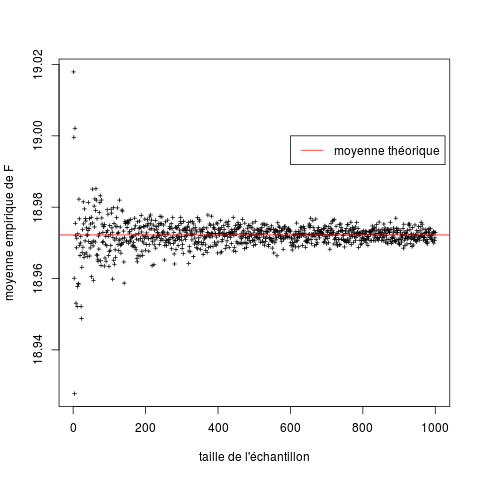
\includegraphics[scale=0.7]{LFGN_F.png}
    \caption{LFGN illustrée avec F}
    \label{LFGN_F}
\end{center}
\end{figure}
\begin{figure}[!h]
\begin{center}
    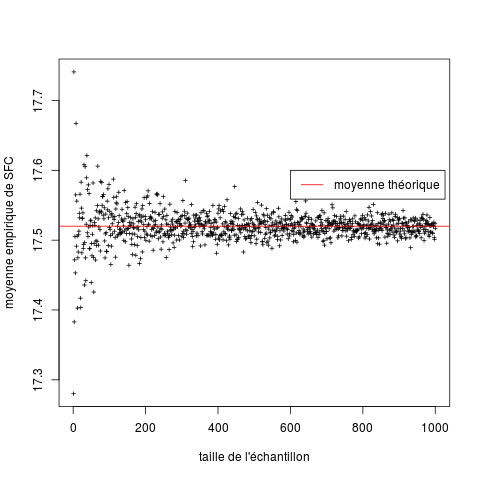
\includegraphics[scale=0.7]{LFGN_SFC.png}
    \caption{LFGN illustrée avec SFC}
    \label{LFGN_SFC}
\end{center}
\end{figure}


\subsection{Théorème central limite}
\begin{theo}[Théorème Central Limite (TCL)]Soit \begin{math}(X_{i})_{i\in\mathbb{N}^{*}}\end{math} des variables aléatoires indépendantes et identiquement distribuées de variance finie \begin{math}\sigma^{2}\end{math} alors
\[\sqrt{n}\left(\frac{\bar{X}_{n}-\mathbb{E}(X_{1})}{\sigma}\right)\xrightarrow[\text{$n\to+\infty$}]{\mathcal{L}}\mathcal{N}(0,1)\]
\end{theo}

Graphiquement, ce théorème signifie que pour un $N$ grand, l'histrogramme décrivant la répartition de la réalisation d'un $K$-échantillon de la variable $\bar{X}_{N}$ suit la courbe de la densité d'une $\mathcal{N}(\mathbb{E}(X_1),\sigma/\sqrt{N})$. 

Les graphes en figures ~\ref{TCL_V}, ~\ref{TCL_F}, ~\ref{TCL_SFC}  illustrent le TCL avec les trois variables du problèmes \footnote{L'échelle de l'axe des ordonnées (fréquence) est étrange car supérieure à 1. Elle est générée automatiquement par R à partir du moment où on utilise la commande \texttt{proba=T} dans \texttt{hist}. Cette bizarrerie irrésolue n'empêche pas la compréhension des graphes.}. L'histogramme ~\ref{TCL_V} représente la répartition de $K$ réalisations de $\bar{V}_N$ ($\sigma=2.309$), l'histogramme ~\ref{TCL_F} la répartition de $K$ réalisations de $\bar{F}_N$ ($\sigma=0.046$) et l'histogramme ~\ref{TCL_SFC} la répartition de $K$ réalisations de $\bar{SFC}_N$ ($\sigma=0.2899$). On constate que la courbe verte représentant la densité d'une loi normale $\mathcal{N}(\mathbb{E}(), \sigma/\sqrt{N})$ épouse bien le contour des histogrammes, conformément au théorème. ($K=1000$ et $N=1000$).

\begin{figure}[!h]
\begin{center}
    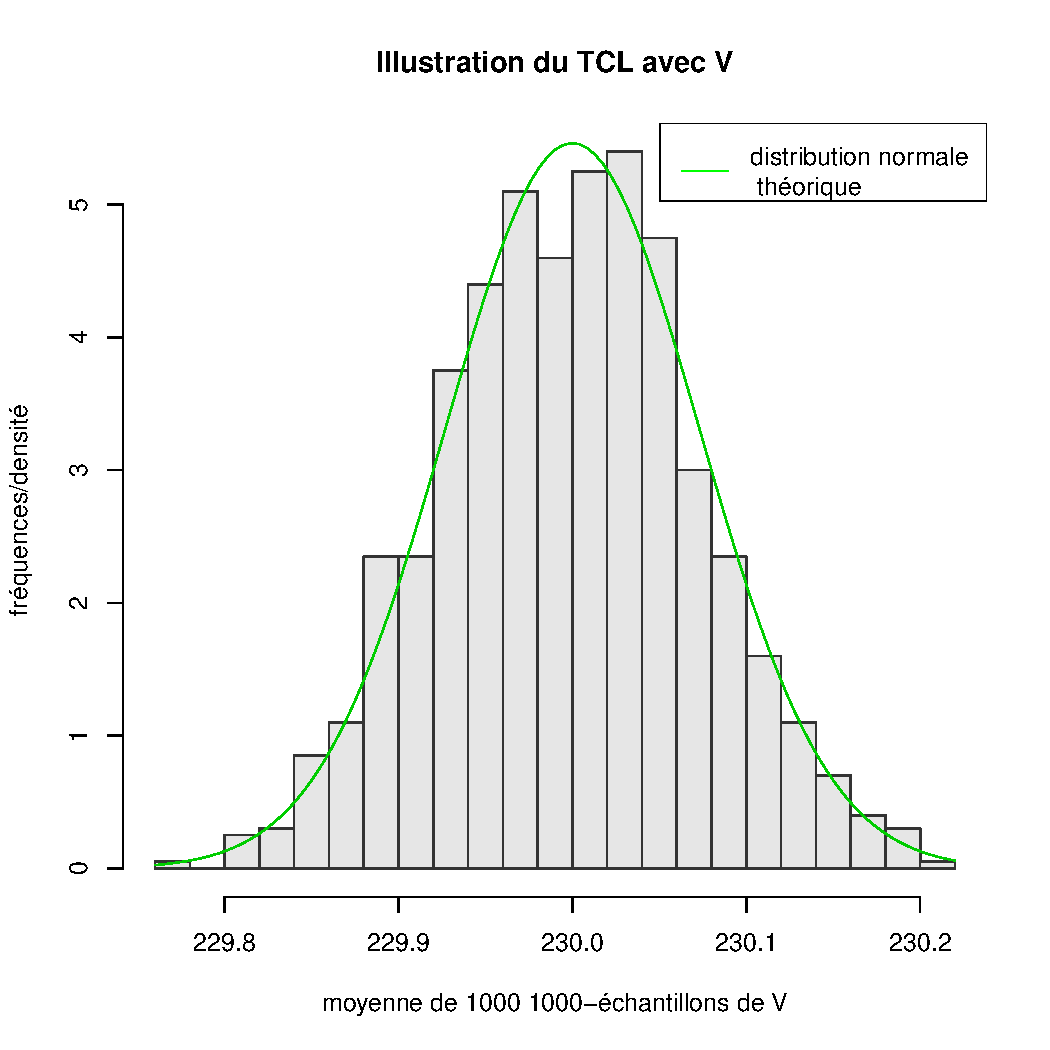
\includegraphics[scale=0.7]{TCLv2_V.pdf}
    \caption{Histogramme de la répartition de $\sqrt{N}\left(\frac{\bar{V}_{N}-\mathbb{E}(V)}{\sigma}\right)$ avec $N=1000$, $\mathbb{E}(V)=230$ et $\sigma=2.309$}
    \label{TCL_V}
\end{center}
\end{figure}
\begin{figure}[!h]
\begin{center}
    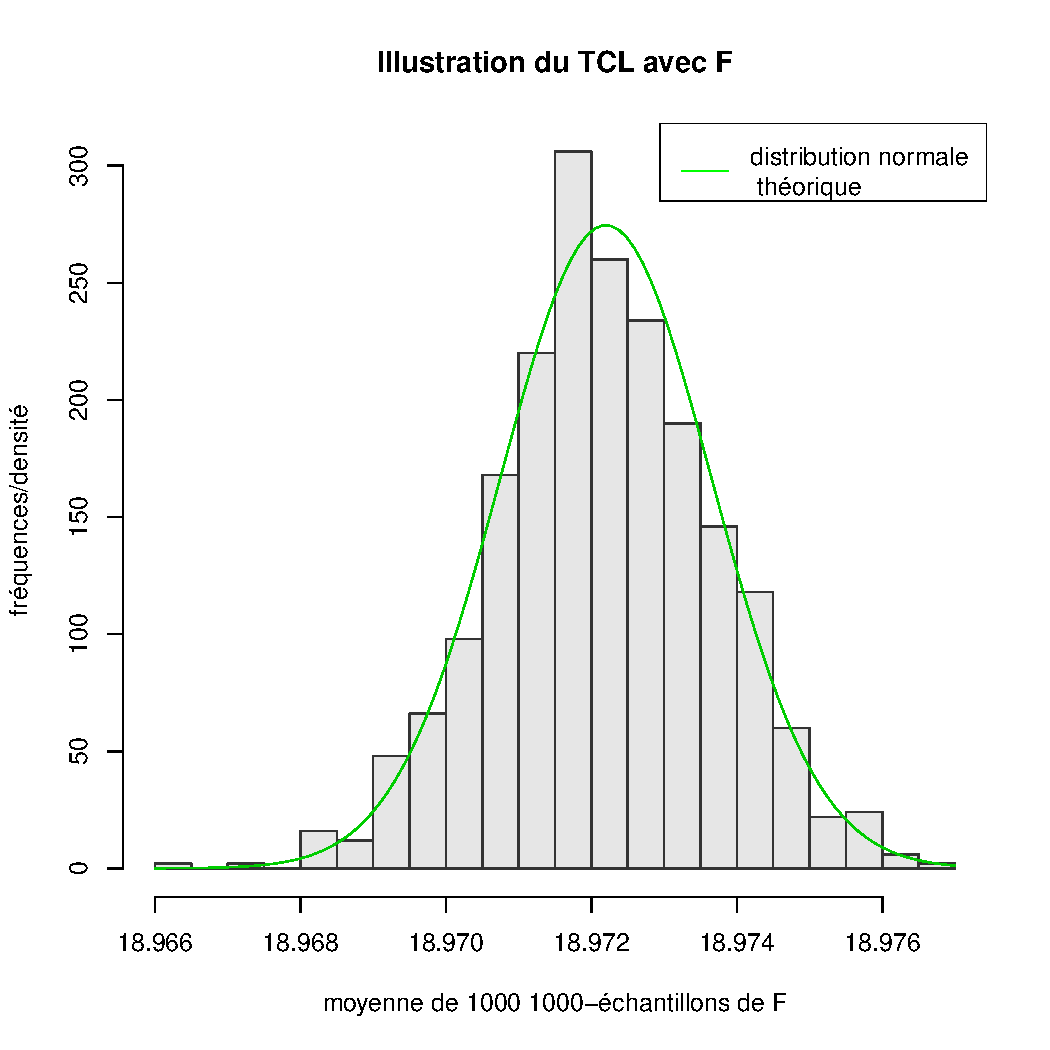
\includegraphics[scale=0.7]{TCLv2_F.pdf}
    \caption{Histogramme de la répartition de $\sqrt{N}\left(\frac{\bar{F}_{N}-\mathbb{E}(F)}{\sigma}\right)$ avec $N=1000$, $\mathbb{E}(F)=18.97$ et $\sigma=0.046$}
    \label{TCL_F}
\end{center}
\end{figure}
\begin{figure}[!h]
\begin{center}
    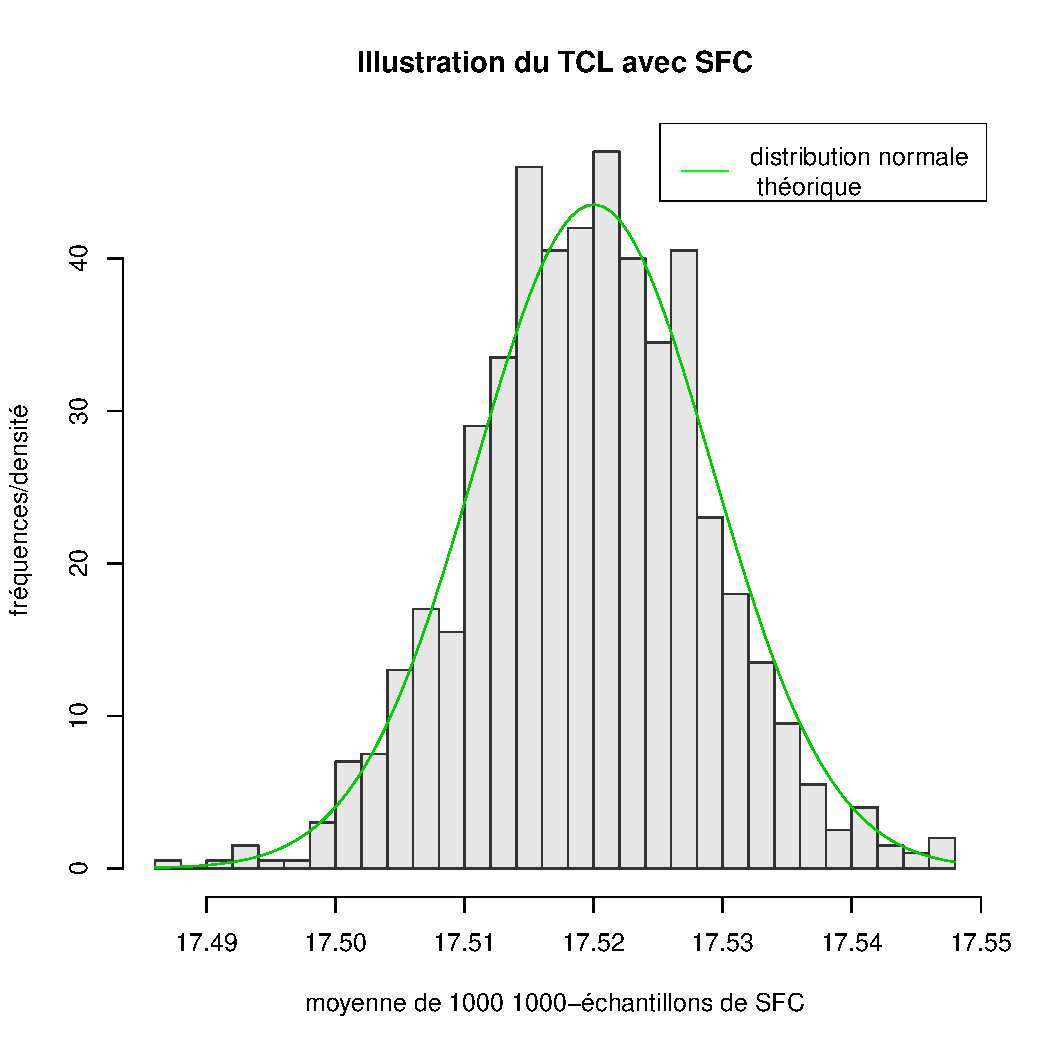
\includegraphics[scale=0.7]{TCLv2_SFC.pdf}
    \caption{Histogramme de la répartition de $\sqrt{N}\left(\frac{\bar{SFC}_{N}-\mathbb{E}(SFC)}{\sigma}\right)$ avec $N=1000$, $\mathbb{E}(SFC)=17.52$ et $\sigma=0.2899$}
    \label{TCL_SFC}
\end{center}
\end{figure}


\subsection{Bruit gaussien}
On suppose que les variables $V$, $F$, et $SFC$ sont bruitées :  
\[V_{i}^{\sigma} = V_i + \sigma \epsilon _i\]
\[F_{i}^{\sigma} = F_i + \sigma \mu _i\]
\[V_{i}^{\sigma} = V_i + \sigma \theta _i\]
où les variables $(\epsilon _i)_{1...N}$, $(\mu _i)_{1...N}$ et $(\theta _i)_{1...N}$ sont iid de loi $\mathcal{N}(0,1)$


Avant d'étudier l'impact du bruit sur $M_{fuel}$, étudions $M_{fuel}$ sans le bruit. On génére pour cela les réalisations d'un $N$-échantillon de $V$, $SFC$, $F$ et on utilise la formule de \textsc{Breguet}. On obtient alors : 
\begin{center}
\begin{tabular}{ | c | c |  c | c |c|c|}
\hline			
   Variable & Moyenne empirique & Variance empirique & Ecart-type empirique & Min & Max\\\hline
   $M_{fuel}$  & 13626.60& 85746.17 & 292.82 & 13141.29 & 15336.92\\
\hline
\end{tabular}
\captionof{table}{Données empiriques simulées sur $M_{fuel}$}
\end{center}
En figure ~\ref{histo_M} est montré l'histogramme de la répartition de 10000 valeurs de $M_{fuel}$ calculées grâce au script \texttt{description.R}. Le trait noir plein est la densité estimée par le logiciel R.
\begin{figure}[!h]
\begin{center}
    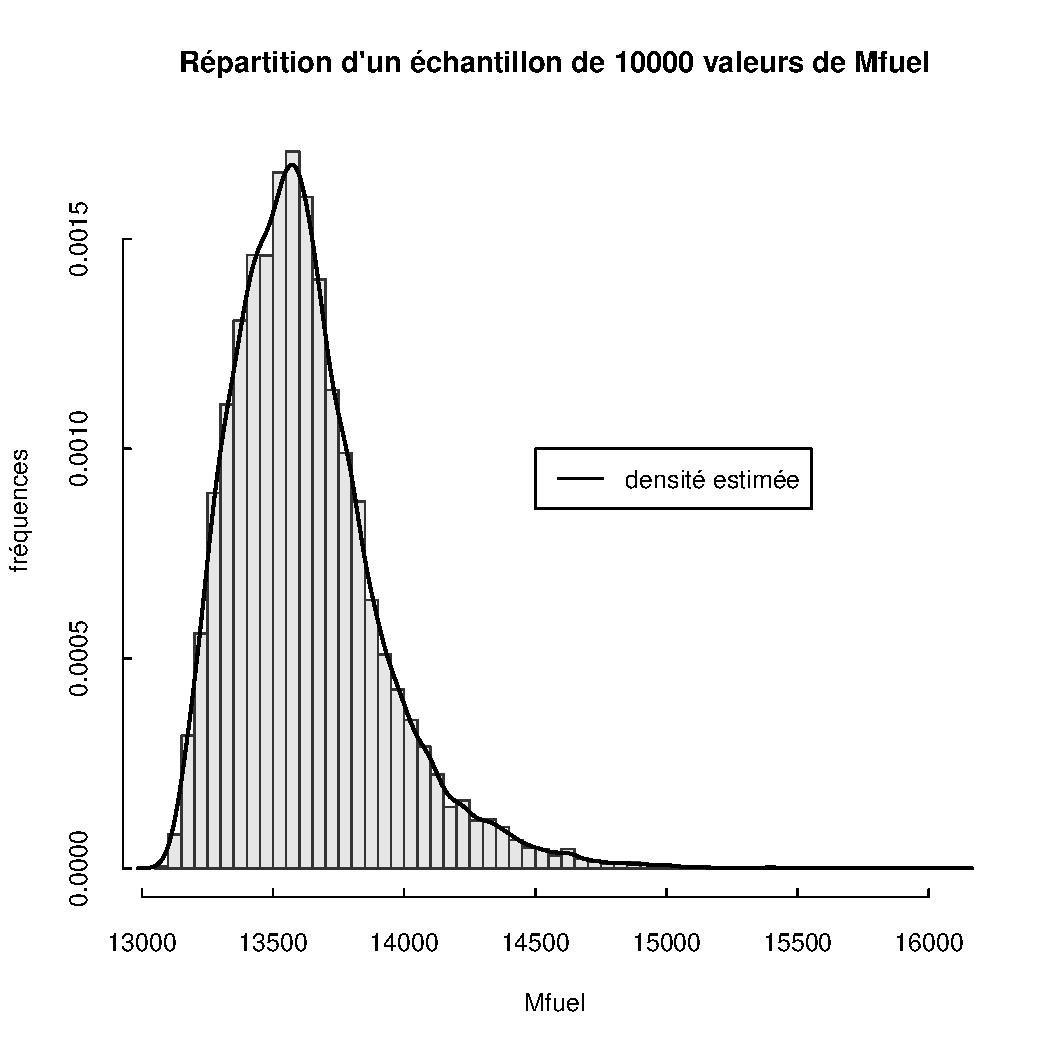
\includegraphics[scale=0.7]{histo_Mfuel.pdf}
    \caption{Histogramme de la répartition de $10000$ valeurs de $M_{fuel}$}
    \label{histo_M}
\end{center}
\end{figure}
\medbreak
Définissons la fourchette du niveau de bruit qui sera étudiée. On peut faire l'hypothèse que le bruit à le même ordre de grandeur que les variances des trois variables. Un bruit trop grand représenterait des variations excessives et peu réalistes (si par exemple le bruit représente les imprécisions de mesures) ; un bruit trop petit serait transparent dans la variation de la variable aléatoire. Ainsi, on choisit d'étudier un bruit tel que $\sigma ^2$ soit compris entre 0.01 et 1.

On constate que plus $\sigma ^2$ augmente, plus la variance empirique de $M_{fuel}$ augmente. De plus, l'écart interquartile augmente. Ces observations rendent compte d'un étalement des réalisations de  $M_{fuel}$. Il est naturel de s'attendre à une dispertion des valeurs si les variables d'entrée sont bruitées. La moyenne, elle, ne varie pas de manière significative. Ceci est certainement dû au fait que les termes d'erreur additionnels soient centrés.  

\begin{center}
\begin{tabular}{ | c | c |  c | c |c|c|}
\hline			
   $\sigma ^2$ & Moyenne empirique & Variance empirique & Min & Max & IQR\\\hline
   0. &13625.85 & 80935.46 & 13100.87 & 15865.00 &  329.37\\
   0.01 & 13619.93&  83323.06& 13079.66& 15810.94 & 336.69\\
   0.05 & 13617.16& 81691.08 & 13009.39 &  15624.84 & 336.24\\
   0.1 &13621.04 & 94345.53 & 12767.53 & 15647.32 &  375.83\\
   0.5 & 13643.27& 390720.59 & 11578.99 & 16670.52 & 836.83\\
   1 &13664.67 & 1356399.4 & 9593.62 & 19579.52 & 1560.89\\
\hline
\end{tabular}
\captionof{table}{Variation des caractéristiques de $M_{fuel}$ en fonction du bruit $\sigma$}
\end{center}
Les résultats ont été obtenus avec des échantillons de taille 10000 pour obtenir une meilleure précision, qui s'amoindrit sinon à cause du bruit.

La figure ~\ref{histo_M_b} montre les différentes densités de $M_{fuel}$ estimées par R pour différents niveaux de bruit. On peut là aussi remarquer un étalement de la densité autour d'une même moyenne qui croit si le bruit augmente ce qui traduit bien la présence de bruit dans les valeurs et illustre les résultats du tableau.


\begin{figure}[!h]
\begin{center}
    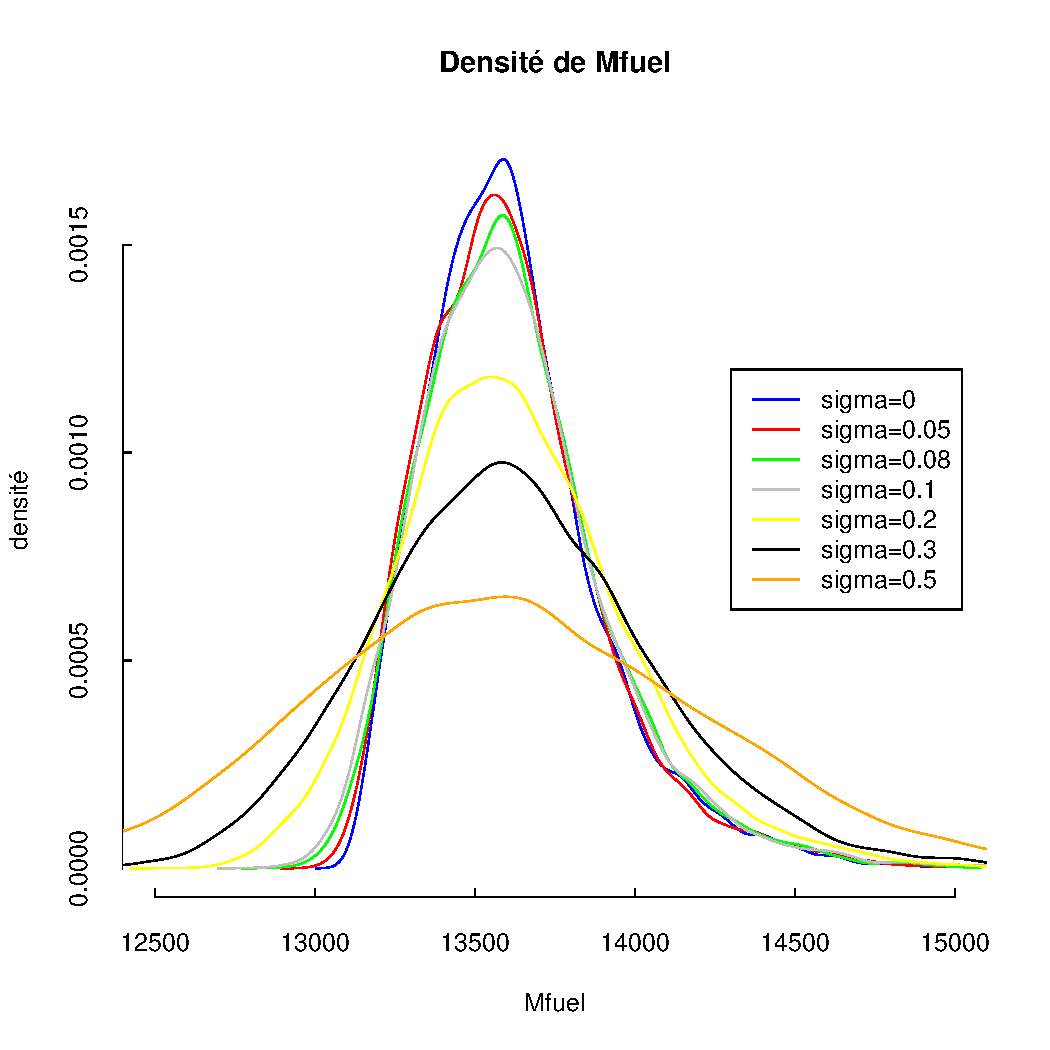
\includegraphics[scale=0.7]{histo_Mfuel_b.pdf}
    \caption{Densité de $M_{fuel}$ pour différents niveaux de bruit. Estimation avec $N=10000$}
    \label{histo_M_b}
\end{center}
\end{figure}
\subsection{Conclusion}
Cette partie théorique a permi d'illustrer deux théorèmes fondamentaux des probabilités et de confronter des valeurs expérimentales sur les échantillons obtenues à partir d'estimateurs classiques avec les valeurs théoriques. 

Pour aller plus loin, on pourrait se demander quelle loi de probabilité correspondrait le mieux pour décrire $M_{fuel}$, à l'aide par exemple d'un test du $\chi^{2}$. On peut penser dans un premier temps vu la forme de la densité que $M_{fuel}$ suit une loi normale centrée sur 13625.85 de variance 80935.46.

On peut aussi constater que $M_{fuel}$ est peu sensible à un bruit faible ($\sigma^2\approx 0.01$) mais beaucoup plus pour un bruit de l'ordre de $\sigma^2\approx 0.5$.

En annexe se trouve des boîtes-à-moustaches de la répartition des valeurs de $M_{fuel}$ afin de rendre plus visuel l'étalement des valeurs à partir d'un bruit élevé. 
\section{Indices de Sobol}
On peut tenter de connaître et quantifier la part d'influence de chacune des variables $V$, $F$, $SFC$ sur $M_{fuel}$ dans la relation $M_{fuel}=f(V, S, SFC)$. Pour détecter les variables les plus influentes, on va s'intéresser aux indices de Sobol $S$. Plus particulièrement, on s'intéressera à l'influence de $F$ et $SFC$ dans notre étude. On cherche alors à estimer simultanément 2 indices de Sobol
\[S:=(S^{\{F\}}, S^{\{SFC\}})=\left(\frac{\text{var}(\mathbb{E}[M_{fuel}|F])}{\text{var}(M_{fuel})},\frac{\text{var}(\mathbb{E}[M_{fuel}|SFC])}{\text{var}(M_{fuel})}\right)\]
à l'aide la méthode \textsc{pick-freeze}.
\subsection{Méthode \textsc{pick-freeze}}
La méthode \textsc{pick-freeze} est une méthode, présentée dans \cite{ref2}, qui permet d'estimer $S$. On présente ici la méthode générale et ses résultats théoriques adaptés à notre problème.

Soit $X=(F, SFC)$ et $X'=(F', SFC')$ une copie indépendante de $X$. On construit alors les vecteurs \textsc{pick-freeze} de la manière suivante : 
\[X^{\{F\}}=(V',F, SFC')\]
Ici, on gèle les valeurs de $F$ et on regénère les valeurs de $V$ et $SFC$.
\[X^{\{SFC\}}=(V',F', SFC)\]
Ici, on gèle les valeurs de $SFC$ et on regénère les valeurs de $V$ et $F$.

Puis on calcule
\[M_{fuel}=f(X)\]
\[M_{fuel}^{\{F\}}=f(X^{\{F\}})\]
\[M_{fuel}^{\{SFC\}}=f(X^{\{SFC\}})\]

Pour estimer $S$, on réalise un $N$-échantillon de $X$ puis on construit à partir de $X$ les $N$-échantillons de $X^{\{F\}}$ et de $X^{\{SFC\}}$ puis on calcule les $N$-échantillons de $M_{fuel}$, de $M_{fuel}^{\{F\}}$ et de $M_{fuel}^{\{SFC\}}$. 

On estime $S$ par les estimateurs suivants : 
\[S^{\{F\}}_{N} = \frac{\frac{1}{N}\sum M_{fuel,i}M_{fuel,i}^{\{F\}} - (\frac{1}{N}\sum M_{fuel,i})(\frac{1}{N}\sum M_{fuel,i}^{\{F\}})}{\frac{1}{N}\sum M_{fuel,i}^{2} - (\frac{1}{N}\sum M_{fuel,i})^{2}}\]
\[S^{\{SFC\}}_{N} = \frac{\frac{1}{N}\sum M_{fuel,i}M_{fuel,i}^{\{SFC\}} - (\frac{1}{N}\sum M_{fuel,i})(\frac{1}{N}\sum M_{fuel,i}^{\{SFC\}})}{\frac{1}{N}\sum M_{fuel,i}^{2} - (\frac{1}{N}\sum M_{fuel,i})^{2}}\]
\[S_N=\left(S^{\{F\}}_{N}, S^{\{SFC\}}_{N}\right)\]

On sait que $S_N$ converge presque sûrement vers $S$. Par conséquent quand $N$ est grand, les réalisations de $S_N$ tendent vers $S$. Ceci est montré grâce aux courbes ~\ref{sobol_F} et ~\ref{sobol_SFC}. 

On retiendra alors une réalisation de $S^{\{F\}}_{N}$ et de $S^{\{SFC\}}_{N}$ pour $N=1000$ :
\[S^{\{F\}}=0.0424\]
\[S^{\{SFC\}}=0.7266\]
En particulier, il semble que 
\[S^{\{F\}} < S^{\{SFC\}}\]
ce qui signifie que $SFC$ a plus d'influence que $F$ dans $M_{fuel}$. Ceci sera discuté dans la partie suivante.

NOTE : il arrive que $S^{\{F\}}_{N} < 0$ alors qu'un indice de Sobol est toujours positif. 

\begin{figure}[!h]
\begin{center}
    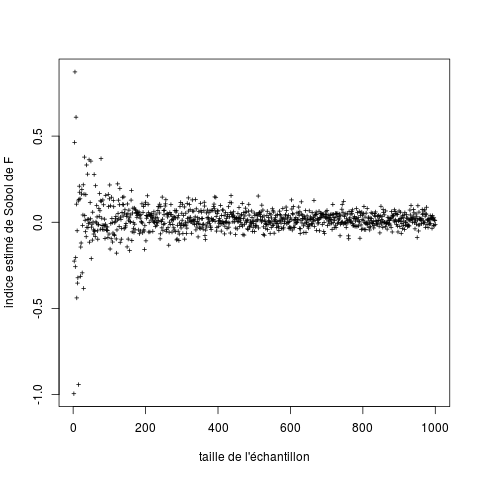
\includegraphics[scale=0.7]{Sobol_F.png}
    \caption{Nuage de points des estimations de $S^{\{F\}}$ en fonction de $N$, taille de l'échantillon}
    \label{sobol_F}
\end{center}
\end{figure}
\begin{figure}[!h]
\begin{center}
    \includegraphics[scale=0.7]{Sobol_SFC.png}
    \caption{Nuage de points des estimations de $S^{\{SFC\}}$ en fonction de $N$, taille de l'échantillon}
    \label{sobol_SFC}
\end{center}
\end{figure}

\medbreak
On constate aussi que lorsque le bruit $\sigma$ augmente, les indices $S^{\{F\}}$ et $S^{\{SFC\}}$ varient. En particulier, $S^{\{F\}}$ augmente et $S^{\{SFC\}}$ diminue comme illustré sur la figure ~\ref{sobol_b}. Avec un bruit important, il devient plus difficile de considérer avec certitude que $S^{\{F\}} < S^{\{SFC\}}$. Cela traduit bien le fait que plus les valeurs d'entrée sont bruitées, plus il est difficile de savoir avec certitude quelle variable a le plus d'influence sur la sortie. 
\begin{figure}[!h]
\begin{center}
    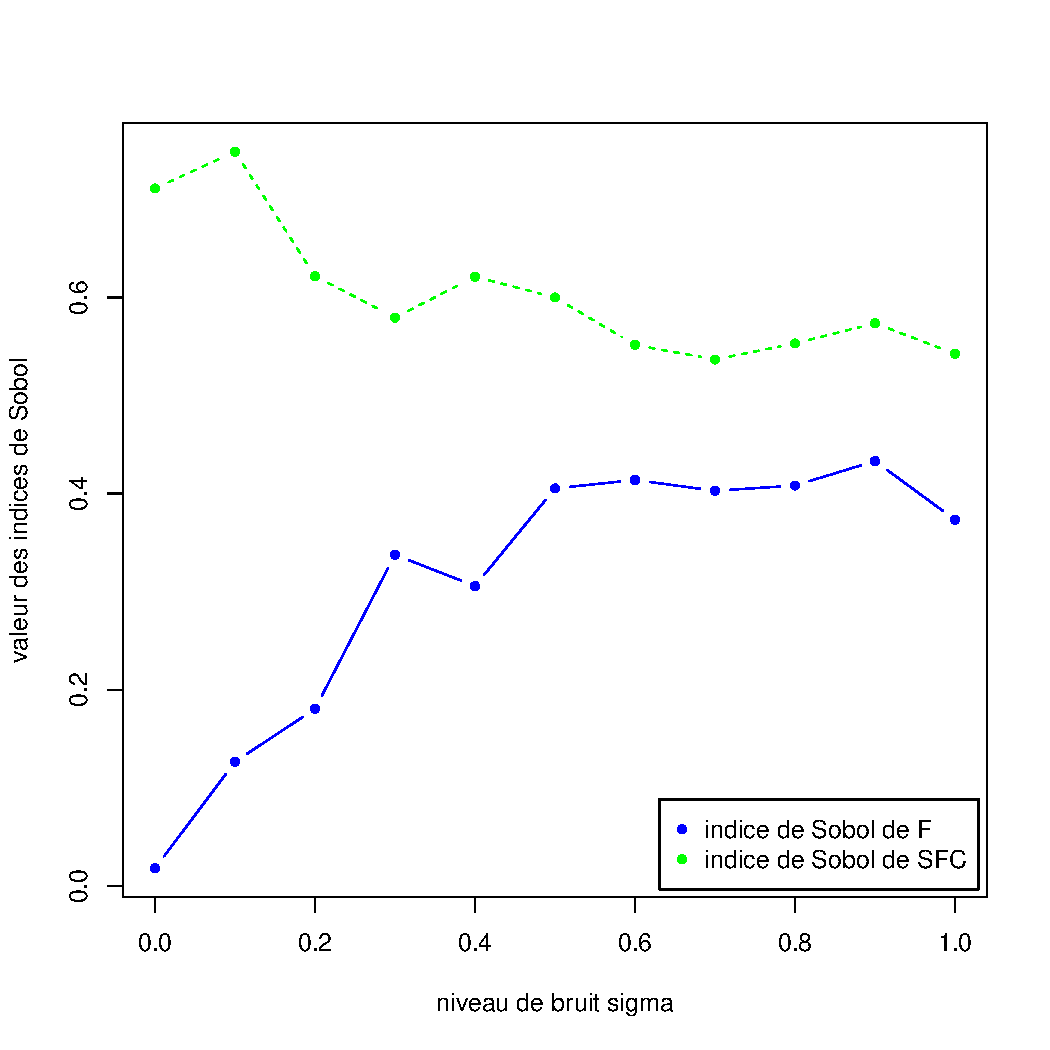
\includegraphics[scale=0.7]{Sobol_b.pdf}
    \caption{Evolution de $S^{\{SFC\}}$ et de $S^{\{F\}}$ en fonction de $\sigma$. $N=10000$}
    \label{sobol_b}
\end{center}
\end{figure}
\subsection{Test}
Une question à se poser pour optimiser la consommation d'un avion est s'il vaut mieux améliorer le moteur ($SFC$) ou l'aérodynamisme ($F$). On cherche donc à savoir quelle variable à le plus d'influence sur $M_{fuel}$. On cherche donc à savoir si $S^{\{F\}} < S^{\{SFC\}}$ ou l'inverse.

Avec la méthode \textsc{pick-freeze}, il semble clair que $S^{\{F\}} < S^{\{SFC\}}$. Mais on va tout de même réaliser un test statistique pour s'en assurer (après tout, $S^{\{F\}}$ et $S^{\{SFC\}}$ restent des estimateurs).

On réalise alors le test suivant :
\[H_{0} : S^{\{SFC\}} \ge S^{\{F\}} \text{ contre } H_{1} : S^{\{SFC\}} < S^{\{F\}}\]

On rejette $H_0$ ssi $S^{\{SFC\}} - S^{\{F\}} < -K$ où $K$ est choisit pour avoir un test de taille $\alpha$. De plus, on se place sous l'hypothèse la moins favorable, c'est-à-dire, $S^{\{SFC\}} - S^{\{F\}} = 0$ (point de $H_0$ le plus proche de $H_1$).

On cherche maintenant la loi asymptotique de $S^{\{SFC\}}_N - S^{\{F\}}_N$ sous l'hypothèse que $S^{\{SFC\}} - S^{\{F\}} = 0$.

On sait par \cite{ref2} que : 
\[\sqrt{N}\left(\begin{pmatrix}S^{\{F\}}_N\\S^{\{SFC\}}_N\end{pmatrix} - \begin{pmatrix}S^{\{F\}}\\S^{\{SFC\}}\end{pmatrix}\right)\xrightarrow[\text{$n\to+\infty$}]{\mathcal{L}}\mathcal{N}_{2}(0,\Gamma)\]
où $\Gamma$ est la matrice 2$\times$2 décrite dans l'annexe.

On applique alors la delta-méthode avec la fonction $h(x,y)=y-x$ dont la jacobienne est $A := \begin{pmatrix}-1 & 1\end{pmatrix}$ pour obtenir (toujours sous l'hypothèse $S^{\{SFC\}} - S^{\{F\}} = 0$) :
\[\sqrt{N}\left(S^{\{SFC\}}_N - S^{\{F\}}_N\right)\xrightarrow[\text{$n\to+\infty$}]{\mathcal{L}}\mathcal{N}(0,\sigma^{2})\]
avec 
\[\sigma^{2}=A\Gamma A^{T}\]
On construit alors un estimateur $\widehat{\sigma^{2}}_N$ convergent de $\sigma^{2}$ en remplaçant dans la matrice $\Gamma$ les indices de Sobol par leur estimateur respectif et les covariances par leur estimateur classique :
\[\widehat{\text{cov}_N}(X, Y) = \frac{1}{N-1}\sum_{i=1}^N (X_i - \bar{X}_N)(Y_i - \bar{Y}_N)\]
Par le théorème de \textsc{Slutsky} : 
\[\sqrt{N}\left(\frac{S^{\{SFC\}}_N- S^{\{F\}}_N}{\sqrt{\widehat{\sigma^{2}}_N}}\right)\xrightarrow[\text{$n\to+\infty$}]{\mathcal{L}}\mathcal{N}(0,1)\]
On en déduit $K$:
\[K=-\frac{\Phi^{-1}(\alpha)\sqrt{\widehat{\sigma^{2}}_N}}{\sqrt{N}}\]
où $\Phi$ est la fonction de répartition de la loi normale.

Ainsi, on rejette $H_0$ ssi $S^{\{SFC\}}_N - S^{\{F\}}_N < \frac{\Phi^{-1}(\alpha)\sqrt{\widehat{\sigma^{2}}_N}}{\sqrt{N}}$
\medbreak
Le sript \texttt{Sobol.R} propose de réaliser le test présenté ci-dessus. 
En voici une expérience :
\begin{center}
\begin{tabular}{ | c | c |  c | c |c|c|}
\hline			
   bruit : $\sigma ^2$ & $S^{\{F\}}$ & $S^{\{SFC\}}$ & niveau : $\alpha$ & seuil & rejet\\\hline
   0 & 0.04762211 & 0.76175453 & 0.05 & -3.71894734 &  FALSE\\
\hline
\end{tabular}
\captionof{table}{Résultat du test}
\end{center}

CONCLUSION : on ne peut pas rejeter l'hypothèse $H_0$.

\medbreak
On peut également répéter cette expérience de niveau $\alpha = 0.05$ 1000 fois et compter le nombre de rejets de $H_0$ pour vérifier la robustesse de ce test. Le script \texttt{Sobol.R} permet de faire cela et on constate qu'on ne peut pas rejeter $H_0$ 1000 fois. Or, le test étant de niveau $0.05$, on s'attend à obtenir environ 50 rejets de $H_0$. Cependant, il ne faut pas oublier que le test a été fait sous l'hypothèse $S^{\{SFC\}} - S^{\{F\}} = 0$. Et on n'a vu que $S^{\{SFC\}} > S^{\{F\}}$. Par conséquent en augmentant le niveau $\alpha$ du test, de plus en plus de tests échoueraient. En effet, avec $\alpha=0.1$, il y a $0\%$ de rejet, avec $\alpha=0.5$, il y a $0\%$ de rejet, pour $\alpha=0.6$, il y a $0.5\%$ de rejet, avec $\alpha=0.61$, il y a $5.3\%$ de rejet et avec $\alpha=0.7$, il y a $100\%$ de rejet. 

Pour tester la robustesse du test, on peut bruiter les variables d'entrées pour s'assurer d'avoir toujour $S^{\{SFC\}} > S^{\{F\}}$. On sait déjà que $S^{\{SFC\}}$ diminue et que $S^{\{F\}}$ augmente lorsque le bruit $\sigma$ augmente. Pour $\sigma$ variant entre $0.01$ et $1$ et $\alpha = 0.05$, il y a $0\%$ de rejet (tests réalisés avec le même script \texttt{Sobol.R}). On en déduit la robustesse du test et qu'on ne peut absolument pas rejeter $H_0$.
\subsection{Conclusion}
Cette partie permet de savoir quelle variable entre $S$ et $SFC$ a le plus d'influence sur $M_{fuel}$ grâce aux indices de Sobol. La méthode \textsc{Pick-Freeze} permet de fournir un estimateur de $(S^{\{F\}}, S^{\{SFC\}})$. Un test, dont l'interprétation est plutôt délicate, permet de conclure qu'on ne peut absolument pas rejeter l'hypothèse selon laquelle $S^{\{F\}} < S^{\{SFC\}}$, même en présence de bruit sur les variables d'entrée. Un constructeur aéronautique peut conclure de cette étude qu'il vaut mieux dépenser pour améliorer le moteur ($SFC$) plutôt que l'aérodynamisme de l'avion ($F$).
\section{Modèle linéaire}
On suppose inconnue la formule de \textsc{Breguet} et on ne dispose que des données $(V_{i}^{\sigma},F_{i}^{\sigma},SFC_{i}^{\sigma}, M_{fuel,i})_{i=1,...,N}$ simulées ($M_{fuel,i}$ est calculé à partir de la formule de \textsc{Breguet}). L'objectif est d'exprimer linéairement $M_{fuel}$ à l'aide de $V$, $F$ et $SFC$ :
\[M_{fuel}=a_{0}+a_{1}V+a_{2}F+a_{3}SFC+u\] $u$ représente une erreure gaussienne indépendante centrée.
\subsection{Estimateurs}
\cite{ref1} propose une méthode pour estimer les coefficients de la régression linaire. En voici les résulats théoriques adaptés à notre problème:

On range les données dans une matrice $\bf{X}$ de $N$ lignes et $4$ colonnes où la première colonne ne contient que de $1$, la deuxième le vecteur des réalisations $(v_{i}^{\sigma})_{i=1,...,N}$, la troisième le vecteur des réalisations $(f_{i}^{\sigma})_{i=1,...,N}$ et la quatrième le vecteur des réalisations $(sfc_{i}^{\sigma})_{i=1,...,N}$ et dans un vecteur $\bf{y}$ composé des réalisations $(m_{fuel,i})_{i=1,...,N}$. On note $\bf{u}$ le vecteur $(u_{1},...,u_{N})^{T}$ des erreurs et $\bf\alpha$ le vecteur $(a_{0},a_{1},a_{2},a_{3})^{T}$. Le problème devient alors :
\[\bf{y}=\bf{X}\bf\alpha+\bf{u}\]
Les estimateurs des $a_{i}$ par la métahode des moindres carrés (MC) est :
\[\bf a=(X^{T}X)^{-1}X^{T}y\]
Il faut pour cela s'assurer que la matrice $X^{T}X$ soit inversible. 

\cite{ref1} donne également les propriétés des estimateurs. En particulier, $\bf a$ est sans biais ($\mathbb{E}(\bf{a})=\alpha$) et efficace (i.e. la matrice de covariance atteint la borne inférieure de Cramer-Rao) sous l'hypothèse de normalité des erreurs. Il faudra obtenir $K$ réalisations de $\bf a$ et les moyenner car rien n'assure la convergence presque sûr de l'estimateur.
\subsection{Estimation des coefficients et des erreurs}
Le fichier \texttt{reg\_lin.R} propose un script R pour calculer les valeurs des $a_{i}$ par la méthode des moindres carrées présentée ci-dessus. A l'aide de la moitié des données $(V_{i}^{\sigma},F_{i}^{\sigma},SFC_{i}^{\sigma}, M_{fuel,i})_{i=1,...,N}$ fixées au départ, on obtient alors :
\[
\left\{
\begin{array}{r c l}
a_{0}=28043.18\\
a_{1}=-62.78\\
a_{2}=-761.42\\
a_{3}=825.64
\end{array}
\right.
\]
On peut s'assurer de la vraissemblance de ces résultats. Constatons d'abord que le signe des coefficients $a_i$ correspond bien au sens de variation de $M_{fuel}$ en fonction de la variable considérée. En effet, si $SFC$ augmente, $M_{fuel}$ augmente aussi et le signe de $a_3$ est positif. De même, $M_{fuel}$ varie dans le sens inverse de $F$ et $V$ et on retrouve bien que les coefficients $a_1$ et $a_2$ sont négatifs. De plus, l'espérance théorique de $M_{fuel}$ selon ce modèle est $a_0+a_1\mathbb{E}(V)+a_2\mathbb{E}(F)+a_3\mathbb{E}(SFC)=13624.85$ ce qui correspond à l'espérance de $M_{fuel}$ calculée en 1.4. De même pour la variance : la variance théorique de $M_{fuel}$ selon ce modèle est $62.78^{2}Var(V)+761.42^{2}Var(F)+825.64^{2}Var(SFC)+\sigma^{2}=79506.42$, ce qui est proche de la variance empirique trouvée en 1.4 avec un bruit de $\sigma^{2}=0.01$, soit $83323.06$ (et aussi $79506.42/83323.06 = 0.9541$, proche de $R^{2}$).

\medbreak
On fixe alors $\alpha$ aux valeurs ci-dessus, et pour la suite, on utilise l'autre moitié des données obtenues.
\medbreak
\cite{ref1} donne également une méthode pour estimer la variance $\sigma_{u}^{2}$ de l'erreur gaussienne $\textbf{u}\sim\mathcal{N}_{N}(0,\sigma_{u}^{2}\mathbb{I})$. Pour cela on utilise l'estimateur sans biais de $\sigma_{u}^{2}$ suivant :
\[\widehat{s^{2}}=\frac{||\bf{y-X\alpha}||^{2}}{N-4}\]
Attention : $N$ est la taille de l'échantillon utilisé pour les calculs. Donc ici, $N$ est égal à la moitié de la taille de l'échantillon de départ.

Le fichier \texttt{reg\_lin.R} propose un script R pour calculer $\sigma_{u}^{2}$. En calculant $\sigma_{u}^{2}$ avec la deuxième moitié de valeurs, on obtient:
\[\sigma_{u}^{2}=14.61\]

Le document \cite{ref1} donne également une méthode pour quantifier la qualité de l'approximation. Pour cela, il faut calculer le coefficient de détermination $R^{2}$. Ce coefficient permet d'exprimer entre 0 et 1 la part de variation de la sortie (ici $M_{fuel}$) expliquée par le modèle linéaire. Avec la deuxième moitié des valeurs et à l'aide du fichier, on trouve que 
\[R^{2}=0.9995\]


Pour discuter de la pertinence de la régression linéaire, on peut regarder le coefficient $R^{2}$. Celui-ci est proche de 1, ce qui signifie qu'une très grande part de la variance de $M_{fuel}$ est expliquée par le modèle : "Plus de $99.9\%$ de la variation de $M_{fuel}$ est expliquée par les variables $V$, $F$, et $SFC$". On peut aussi comparer la valeur de $\sigma^{2}_{u}$ avec la variance estimée de $M_{fuel}$ et des variables $a_1V$, $a_2F$ et $a_3SFC$ (avec l'hypothèse d'un bruit $\sigma^{2}=0.01$ 
\[\text{var}(M_{fuel})=83323.06 \gg  \sigma^{2}_{u}\]
\[\text{var}(a_1V)=21046.69 \gg  \sigma^{2}_{u}\]
\[\text{var}r(a_2F)=7020.89 \gg  \sigma^{2}_{u}\]
\[\text{var}(a_3SFC)=64078.05 \gg  \sigma^{2}_{u}\]
De même :
\[a_{0}=28043.18 \gg \sqrt{\sigma^{2}_{u}}=3.82\]

On peut en conclure que le modèle obtenu grâce à la régression linéaire ne paraît pas absurde. Dans l'annexe se trouve les valeurs de $a_0$, $a_1$, $a_2$ et $a_3$ entourées d'un intervalle de confiance pour rendre ces valeurs plus pertinentes. 
\subsection{Retour sur les indices de Sobol}
On peut estimer les indices de Sobol de $F$ et $SFC$ avec le modèle obtenu précédemment avec un niveau de bruit fixé à  $\sigma=0.01$
\[M_{fuel}=a_{0}+a_{1}V+a_{2}F+a_{3}SFC\]
pour connaître la part de variation de $F$ et de $SFC$ dans ce modèle et les comparer au modèle original.
Le script \texttt{Sobol\_lin.R} estime les différents indices. On a alors :
\[S^{\{F\}}=0.0784\]
\[S^{\{SFC\}}=0.6802\]

Les indices de Sobol obtenus avec la formule de \textsc{Breguet} avec un niveau de bruit de $\sigma=0.01$ sont :
\[S^{\{F\}}=0.0391\]
\[S^{\{SFC\}}=0.7058\]

On constate que les indices calculés avec le modèle linéaire et la formule sont proches. Par conséquent, le modèle linéaire semble traduire la même chose quant à l'influence des variables $F$ et $SFC$ sur $M_{fuel}$ que la formule. Ceci est un argument de plus pour la pertinence du modèle linéaire. 
\subsection{Conclusion}
On a découvert dans cette partie une nouvelle partie des statistiques qui tente d'expliquer une variable par des relations linéaires avec d'autres variables. Un calcul permet de déterminer les coefficients permettant de réaliser une régression linéaire de $M_{fuel}$, expliquée par $V$, $F$ et $SFC$. La modélisation obtenue semble pertinente et s'accorde aux même résulats que la partie 2.
\section{Conclusion générale}
Ce BE a permis de travailler une bonne partie du programme de statistiques (estimateurs, test et analyse de sensibilité) et de découvrir de nouvelles notions comme la régression linéaire. R a été utilisé comme un langage de programmation et certains graphes ont été difficiles à mettre en forme. Nous avons travaillé tous ensemble sur les trois parties et avons mis en commun avant que Elie \textsc{Grenier} ne rédige le rapport en \LaTeX. 

On peut pour aller plus loin supposer que l'on ne dispose que des échantillons de $V$, $F$, et $SFC$ et inférer les lois des variables (par différents test comme \textsc{Kolmogorov-Smirnov} ou \textsc{Shapiro-Wilk}). Dans le même esprit, il semble pertinent de mettre en place des tests afin de tester la normativité de la loi de $M_{fuel}$ qui a été supposée à la partie 1. On peut aussi chercher d'autres modèles explicatifs de $M_{fuel}$ différents de la régression linéaire, comme des régressions non-linéaires ou non-paramétriques. (problèmes d'optimisation afin de minimiser la fonction d'écart au modèle).



\bibliography{bibli}
\bibliographystyle{plain}
\end{document}
